\newgeometry {
    top = 1 in,
    bottom = 1 in,
    left = 0.6 in,
    right = 0.6 in
}

% Give your report a title
\newcommand\reporttitle{\textbf{Mini Project Report}}
\newcommand\group{\textbf{Group - B1}}

% Add an experiment number
% \newcommand\expno{\textbf{Experiment No. 1}}

% Insert course code, name, quartile number, and year (or any other subtitle)
\newcommand\reportsubtitle{
    \textbf{Machine Learning based short-term\\ forecasting of Orange and Cotton crop\\ prices in context of Indian market\\}
}

\begin{titlepage}
    
    \addmargin
    \centering
    % \sffamily

% 
\includegraphics[width=.36\textwidth]{Figures/Logos/YCCE.png}

% \vspace{8 cm}

{\Large \reporttitle}

% {\large \expno}
\vspace{1 em}
on
\vspace{1 em}

{\LARGE \reportsubtitle}

\vspace{4 em}

\begin{table}[H]
    \centering
    % \sffamily
        Submitted by\\
    \large
        \vspace{1 em}
    \begin{tabu} to \linewidth {C C C C C}
        \textbf{Student Name} & \textbf{Enrollment No.} & \textbf{Semester} & \textbf{Section} & \textbf{Roll No.}\\
        Mr. Humanshu D G & 20010635 & VII & B & 147\\
        Mr. Susrut Patole & 20010522 & VII & B & 169\\
        Ms. Neha Thakur & 20010732 & VII & B & 110\\
        Ms. Geetika Mahant & 20010191 & VII & B & 102
    \end{tabu}
\end{table}

\vspace{4 em}

\begin{table}[H]
    \centering
    % \sffamily
        Under the guidance of\\
    \large
        \vspace{1 em}
    \begin{tabu} to \linewidth {C}
        \textbf{Prof. (Dr.) Nileshsingh V. Thakur}
    \end{tabu}
\end{table}

% \tikz[remember picture, overlay, opacity = 0.11]\node[anchor = south, inner sep = 0 pt] at (current page.south) {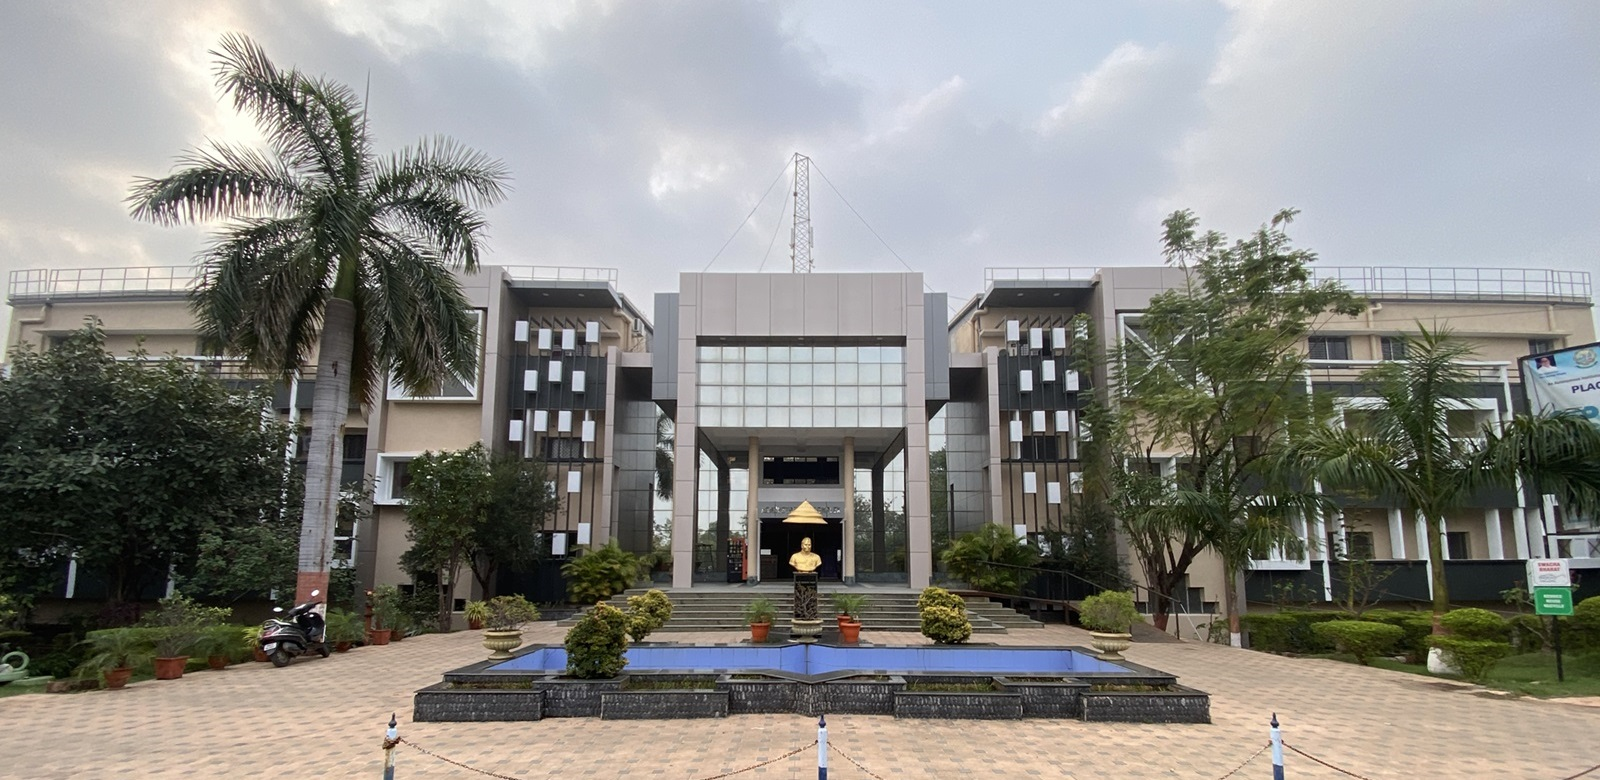
\includegraphics[width=\paperwidth]{Figures/Logos/YCCE Main Building tall.jpg}};

% \tikz[remember picture, overlay]\node[anchor = south, inner sep = 0 pt] at (current page.south) {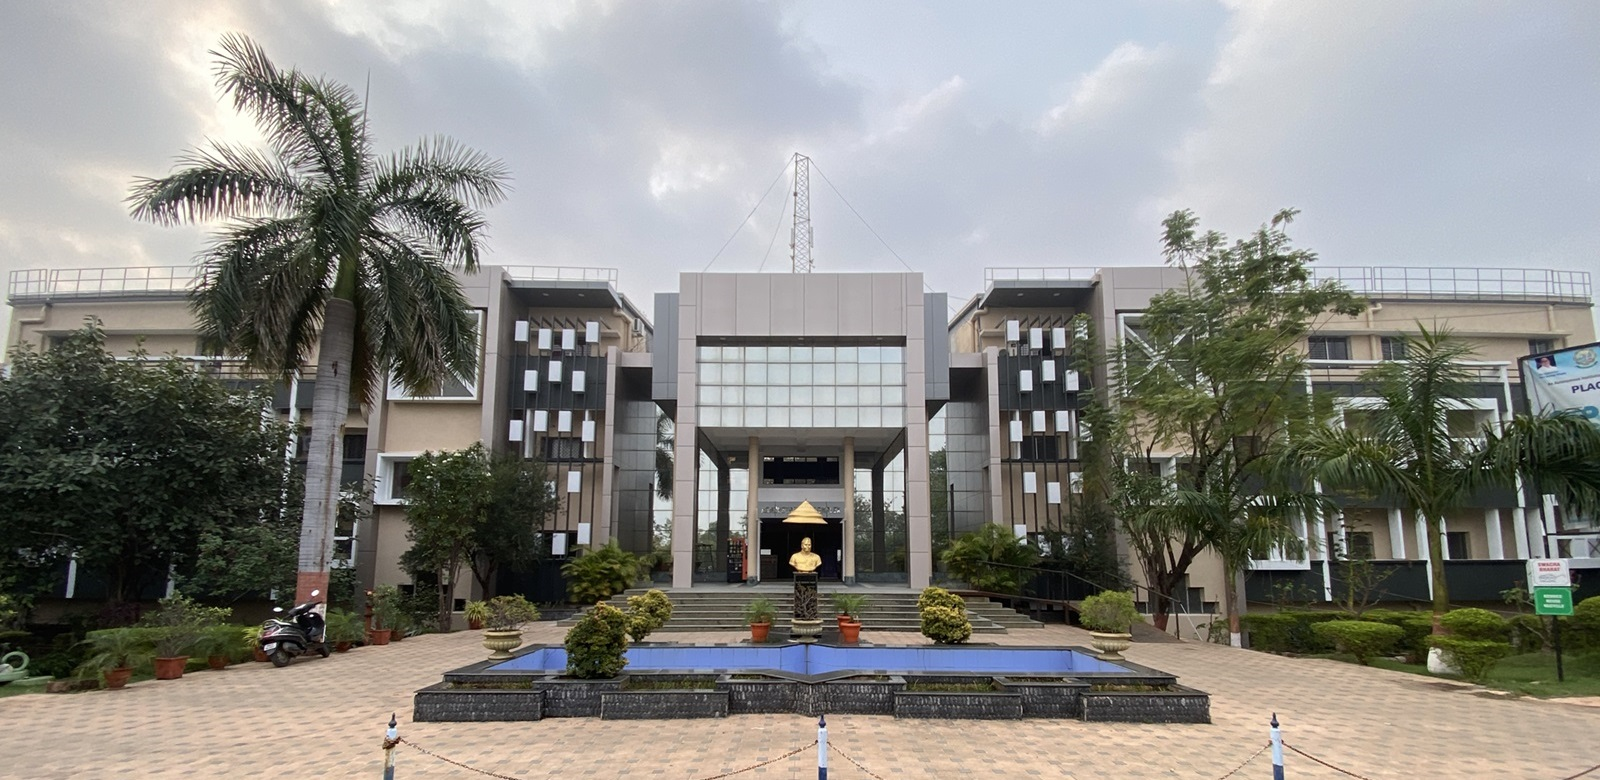
\includegraphics[width=\paperwidth]{Figures/Logos/YCCE Main Building tall.jpg}};

\mbox{}
    \vfill
    % \sffamily
    \large
    \textcolor{white}{\placeanddate}
\end{titlepage}